% !TeX root = ../main/thesis_main.tex
% ---------------------------------------------------
% ----- Chapters of the template
% ----- for Bachelor-, Master thesis and class papers
% ---------------------------------------------------
%  Created by C. Müller-Birn on 2012-08-17, CC-BY-SA 3.0.
%  Freie Universität Berlin, Institute of Computer Science, Human Centered Computing. 
%
\chapter{Kapitel}
\label{chap:chapters} 

\begin{itemize}
	\item Abhängig vom Ziel der Arbeit und dem verwendeten Forschungsdesign unterscheidet sich dieser Hauptteil der Arbeit erheblich. 
	\item Eine sehr allgemeine Struktur ist die folgende:
	\begin{itemize}
		\item Hintergrund der Arbeit (Theoretische Einordnung der Arbeit) 
		 	\begin{itemize}
		 		\item Hier sollte enthalten sein, welche Anwendungen in diesem Bereich bereits existieren und warum bei diesen ein Defizit besteht. 
				\item Falls genutzt, sollten hier die entsprechenden Algorithmen erläutert werden.
				\item Es sollten die Ziele der Anwendungsentwicklung, d.h. die Anforderungen herausgearbeitet werden. Dabei sollte die bestehende Literatur geeignet integriert werden.
		 	\end{itemize}
		\item Umsetzung (Praktischer Anteil der Arbeit)
			\begin{itemize}
				\item Zunächst sollte die Softwarearchitektur und die genutzten Anwendungen, APIs etc. erläutert werden. Ebenfalls gehört dazu das Datenbankschema.
				\item Es sollten die zentralen Elemente der Software (abhängig von der Aufgabenstellung) beschrieben werden, wie implementierte Algorithmen oder das Oberflächendesign.
				\item Zentraler Quellcode sollte entsprechend aufgelistet werden:
				\lstset{language=Java,basicstyle=\footnotesize,numbers=left,showstringspaces=false,frame=single}
				\begin{lstlisting}
				public class Main {
					public static void main(String[] args) {
						System.out.println("Hello World!");
					}
				}
				\end{lstlisting} 
				%\item Klassendiagramm für Backend
				%\item Dr Quellcode zentraler Implementierungen  können als Auszug in den Anhang. Im Text kann dann darauf verwiesen werden.
			\end{itemize}
		\item Evaluation (zumeist nur für Masterarbeiten relevant)
		\begin{itemize}
			\item Jede Software muss auch getestet werden. Dieses Tests werden entweder mit einem vorgegebenen Datensatz erfolgen oder aber die Evaluation erfolgt auf Basis von Experimenten. In diesem Kapitel sollte daher entweder der genutzte Datensatz oder der experimentelle Aufbau beschrieben werden. 
		\end{itemize}
		\item Ergebnis und Diskussion
		\begin{itemize}
			\item Die Ergebnisse der Anwendung werden in diesem Kapitel vorgestellt und anschließend diskutiert. Wenn möglich sollte die Ergebnisse in Relation zu bestehenden Arbeiten in dem Bereich erörtert werden.
		\end{itemize}
	\end{itemize}  
\end{itemize}

\chapter{Literature mapping study}

\section{Motivation}

\section{Methodology}
In order to generate a reproducible and current overview over the fast-moving field of interpretability research in machine learning a rigorous methodology by Peterson et al. \cite{petersenSystematicMappingStudies} is used. 

The recommended process is augmented by further steps in order to tailor it to the existing use case and consists of the following seven procedures:
\begin{enumerate}
	
	\item Definition of research questions:
	The overall process starts by defining clear questions which should guide the development of the whole literature study and subsequently the result as well. Since I am interested in the gaining an overview over the existing interpretability techniques, I chose the following questions:
	
	\begin{enumerate}
		\item What kind of explainability techniques are mentioned in the corpus?
		\item In which domain and for which applications are they most commonly used?
		\item Which techniques are applicable to results produced by the pipeline or the pipeline itself? \tk{Is that right here already?}
	\end{enumerate}
	
	\item Construction of a search string:
	
	Based on the questions one is able to gather a set of key words which are most relevant to the field which is analyzed. Each word is augmented by synonyms which are concatenated with boolean OR operators and several of these synonymous groups are again connected via logical ANDs. Applying this method to the previously found questions yields the following search string:
	
	\textit{( 'explainability' OR 'explainable' OR 'explanation' OR 'interpretability' OR 'interpretable' OR 'interpretation' ) AND ( 'machine learning' OR 'deep learning' OR 'AI' OR 'artificial intelligence')}
	
	
	\item Analysis of the main publishers using a meta search and the search string:
	
	Due to the presumed distributed nature of interpretability research it is not easy to pinpoint the main publishers of scientific articles. In order to mitigate this a pre-search in the meta-search engine 'Google Scholar' is conducted. It should be noted at this point that any biases which are apparent in the meta search engine therefore apply to this analysis as well. One can see in \autoref{fig:publisher_distribution} that the main publishers are respectivly Arxiv, IEEE, Springer and ACM. Since all of these publishers are mainly focused on publications in computer science, mathematics and engineering, this speaks in favor of the hypothesis that most of the research is still very technical and research from social sciences rarely influences it. Even though Arxiv is not a credible publisher per se, it seems like the research community uses it as the first place to publish ones work and therefore it should not be excluded in this analysis. 
	
\begin{pycode}
import pandas as pd
import seaborn as sns
import matplotlib.pyplot as plt
sns.set(style="ticks", color_codes=True)


df = pd.read_csv('../chapters/literature_analysis/data/meta_search.csv')
df = df.groupby(['Publisher']).size().reset_index(name='counts').sort_values(by='counts', ascending=False)
N = 4
topn = df.iloc[:N]
topn.loc['Other'] = [f'{len(df.iloc[N:])} other publishers', df['counts'].iloc[N:].sum()]
g = sns.catplot(x="Publisher", y='counts', kind="bar", palette="ch:.25", data=topn);
g.set_xticklabels(rotation=90)
plt.tight_layout();
plt.savefig("myplot.pdf", bbox_inches="tight");

print(r"\begin{figure}[tbp]")
print(r"\centering")
print(r"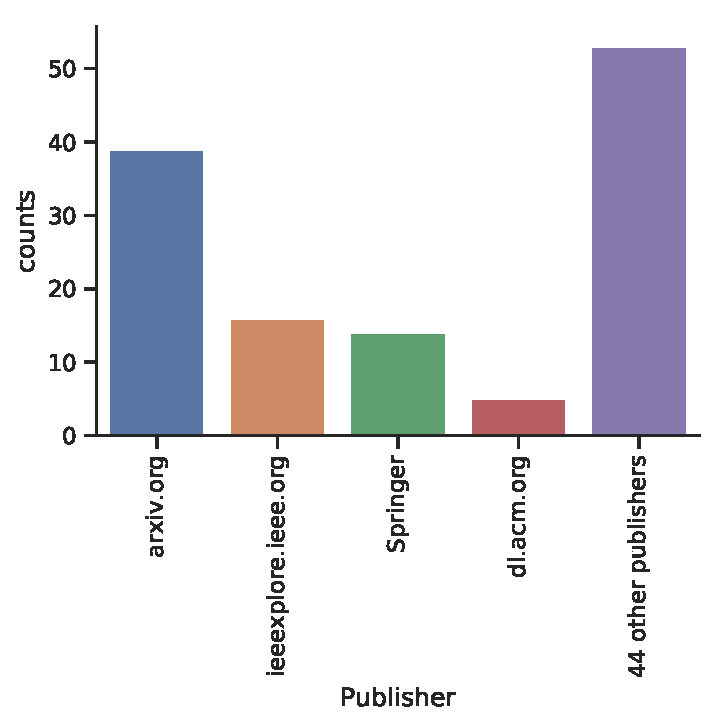
\includegraphics[width=0.65\textwidth]{myplot.pdf}")
print(r"""\caption{\label{fig:publisher_distribution}%
	Barplot displaying the distribution of publishers occurring in the meta search results}""")
print(r"\end{figure}")
\end{pycode}

	\item Sourcing of publications in scientific databases:
	
	Based on the insights from the previous step each of the main publisher's databases is scraped using the search string. Since most searches result in more than 1000 publications only the top 100 results ordered by the relevance scoring of the database are taken into account. These publications are then merged into one corpus.
	
	\item Filtering of these publications by keywording their abstracts
	
	Most scientific databases do a full text search on publications and possibly find the supplied keywords from the search string in parts of the paper which are not relevant e.g. the bibliography. Therefore another filtering step is necessary which searched for the search string in the abstracts of the papers of the corpus.
	
	\item Definition and application of inclusion and exclusion criteria to narrow down the pool of publications further
	
	gg
	\item Quantitative and qualitative assessment of the resulting corpus
\end{enumerate}

